\section{Protocolos}

\begin{frame}{Protocolos}
	\begin{block}{Estructura Google Cast}
		\begin{itemize}
			\item Detección de dispositivos (mDNS)
			\item Intercambio de mensajes (Software propietario)
		\end{itemize}
	\end{block}

	\begin{block}{ }
		La primeras versiones del Chromecast usaban el protocolo DIAL que englobaba ambos pasos.
	\end{block}
\end{frame}


\subsection{DIAL}
\begin{frame}{DIAL}
	\begin{block}{ }
		DIAL (DIscovery And Launch) es el antiguo protocolo de comunicación.
		Se basa en Universal Plug and Play (UPnP), Simple Service Discovery Protocol (SSDP) y protocolos HTTP.

		SSDP sirve para la búsqueda de dispositivos UPnP.
		Utiliza UDP en unicast o multicast en el puerto 1900 para anunciar los servicios de un dispositivo.
	\end{block}

	\begin{block}{ }
		El protocolo DIAL tiene dos componentes
		\begin{itemize}
			\item DIAL Service Discovery
			\item DIAL REST Service
		\end{itemize}
	\end{block}
\end{frame}



\begin{frame}{DIAL Service Discovery}
	\begin{figure}[H]
		\centering
		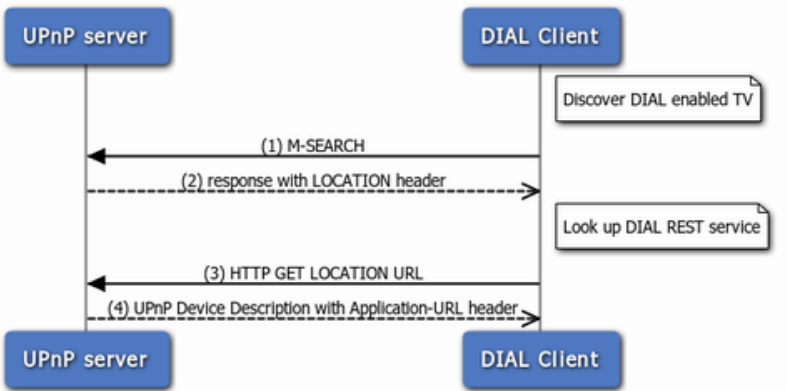
\includegraphics[width=1\textwidth]{./Imagenes/dial.png}
		\label{fig:DIAL}
	\end{figure}
\end{frame}

\begin{frame}{DIAL REST Service}
	\begin{figure}[H]
		\centering
		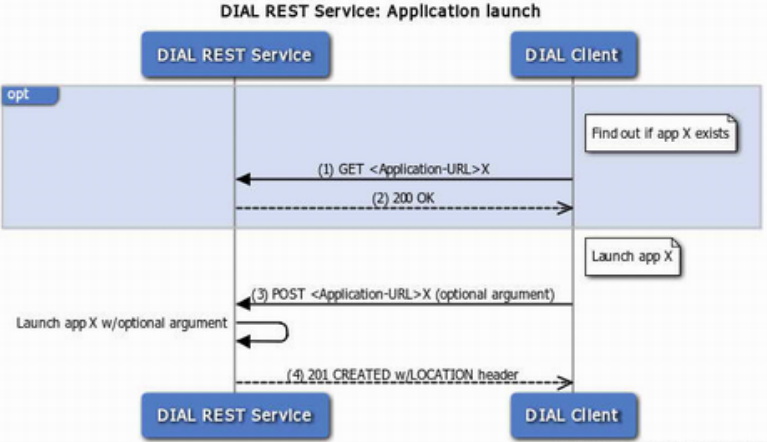
\includegraphics[width=1\textwidth]{./Imagenes/dialrest.png}
	\end{figure}
\end{frame}

\subsection{mDNS}

\begin{frame}{mDNS}
	\begin{block}{mDNS}
		Multicast Domain Name System es la implementación del protocolo de resolución de nombres (DNS) para redes de área local, donde no existe un servidor DNS real.
	\end{block}

	\begin{block}{Ventajas}
		\begin{itemize}
			\item Poca configuracion para activarse
			\item Funciona cuando no hay infraestructura
			\item Soporta fallos en la infraestructura
		\end{itemize}
	\end{block}
\end{frame}


\begin{frame}{Primer paso mDNS}
	\begin{figure}[H]
		\centering
		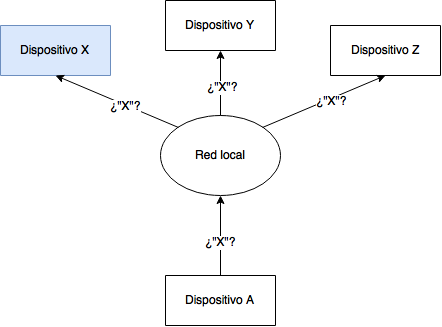
\includegraphics[width=0.75\textwidth]{./Imagenes/mdns1.png}
		\label{fig:mdns1}
		%\caption{Primer paso del protocolo mDNS}
	\end{figure}
\end{frame}


\begin{frame}{Petición}
	\begin{exampleblock}{Ejemplo}
		\centering
		00 00 \textbf<2>{00 00} 00 01 00 00 \hspace{0.1cm} 00 00 00 00  \textbf<3>{07 61 70 70}

		\textbf<3> {6c 65 74 76} \textbf<4>{05 6c 6f 63} \hspace{0.1cm} \textbf<4>{61 6c} 00 00 01 00 01

	\end{exampleblock}

	\begin{itemize}
		\item<1-> Flag de \textbf<2->{petición}
		\item<1-> Nombre de dominio del servidor (\textbf<3>{appletv}.\textbf<4>{local})
	\end{itemize}
\end{frame}


\begin{frame}{Segundo paso mDNS}
	\begin{figure}[H]
		\centering
		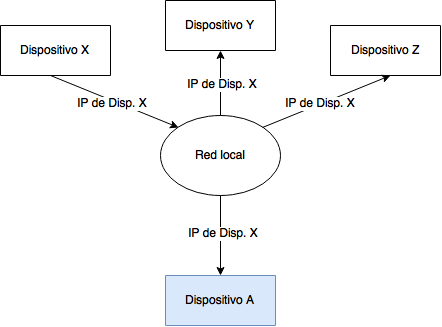
\includegraphics[width=0.75\textwidth]{./Imagenes/mdns2.png}
		\label{fig:mdns2}
		%\caption{Segundo paso del protocolo mDNS}
	\end{figure}
\end{frame}



\begin{frame}{Respuesta}
	\begin{exampleblock}{Ejemplo}
		\centering
		00 00 \textbf<2>{84 00} 00 00 00 01 \hspace{0.1cm} 00 00 00 02 07 61 70 70

		6c 65 74 76 05 6c 6f 63 \hspace{0.1cm} 61 6c 00 00 01 80 01 00

		00 78 00 00 04 \textbf<3>{99 6d 07} \hspace{0.1cm} \textbf<3>{5a} c0 0c 00 1c 80 01 00

		00 78 00 00 10 \textbf<4>{fe 80 00} \hspace{0.1cm} \textbf<4>{00 00 00 00 00 02 23 32}

		\textbf<4>{ff fe b1 21 52} c0 0c 00 \hspace{0.1cm} 2f 80 01 00 00 78 00 00

		08 c0 0c 00 04 40 00 00 \hspace{0.1cm} 08
	\end{exampleblock}

	\begin{itemize}
		\item Flag de \textbf<2>{respuesta}
		\item \textbf<3>{Bytes de dirección IPv4}
		\item \textbf<4>{Bytes de dirección IPv6}
	\end{itemize}
\end{frame}


\subsection{Modo invitado}
\begin{frame}{Modo invitado}
	\begin{block}{ }
		Hasta diciembre de 2014, el dispositivo emisor y receptor debían estar conectados a la misma red
		Wi-Fi. Ya no es necesario gracias al modo invitado.

		En este modo, el receptor emite ultrasonidos por el altavoz reconocidos por el emisor. También puede usarse un PIN de cuatro dígitos para identificación.
	\end{block}


	\begin{block}{Video}
	\href{https://www.youtube.com/watch?v=w6lRq5spQmc}{Ultrasonic Networking using the Web Audio API}
	\end{block}
\end{frame}


\subsection{Comparación otros protocolos}

\subsubsection{Mirascat}

\begin{frame}{Miracast}
	\begin{block}{ }
		Miracast es un protocolo multimedia para hacer streaming a un monitor desde un dispositivo local.

		Con Miracast el dispositivo receptor es dependiente de que el dispositivo Android emisor se mantenga activo: si se bloquea también bloqueará la reproducción en el receptor.
	\end{block}
	
	\begin{block}{Capas}
		\begin{itemize}
			\item Capa de internet: IPv4
			\item Capa de transporte: TCP/UDP
			\item Capa de aplicación, RTSP y RTP
		\end{itemize}
	\end{block}
\end{frame}

\begin{frame}
	\begin{block}{Red}
		La conexión está creada vía Wi-Fi Protected Setup
		(WPS), mecanismos para facilitar la configuración de
		una red WLAN con seguridad WPA2.
		
		Existe una alternativa de código abierto a Miracast llamada \href{https://github.com/albfan/miraclecast}{MiracleCast}.
	\end{block}
	
	\begin{alertblock}{Sin soporte de Google}
		A partir de Android 6.0, Google ha dejado de dar soporte nativo a Miracast en favor de su propio Google Cast.
	\end{alertblock}
\end{frame}

